
\begin{frame}
    \centering
    \textbf{\Large{Density Functional Theory}}
\end{frame}

\begin{frame}
    \frametitle{The molecular Schr\"{o}dinger equation}
    \ \\
    {\large
    \begin{equation}
	\nonumber
	\hat{H}\Psi = E\Psi
    \end{equation}
    }

    \begin{equation}
	\nonumber
	\hat{H} =
        - \sum_I \frac{\nabla^2}{2M_I} - \sum_i \frac{\nabla^2}{2}
	+ \sum_{I>J} \frac{Z_IZ_J}{|\boldsymbol{R}_I-\boldsymbol{R}_J|} 
	- \sum_{i,I} \frac{Z_I}{|\boldsymbol{r}_i-\boldsymbol{R}_I|} 
	+ \sum_{i>j} \frac{1}{|\boldsymbol{r}_i-\boldsymbol{r}_j|} 
    \end{equation}

    \vspace{5mm}

    \centering
    For an $N$-particle problem, the wave function is $3N$-dimensional
    \begin{equation}
	\nonumber
	\Psi = \Psi(\boldsymbol{r}_1,\boldsymbol{r}_2,\dots,\boldsymbol{r}_N)
    \end{equation}

    \vspace{5mm}

    \pause
    \centering
    $\beta$-Carotene ($C_{40}H_{56}$) has 296 electrons and an 888-dimensional wavefunction!
    \only<1>{
    \begin{center}
    %white background
    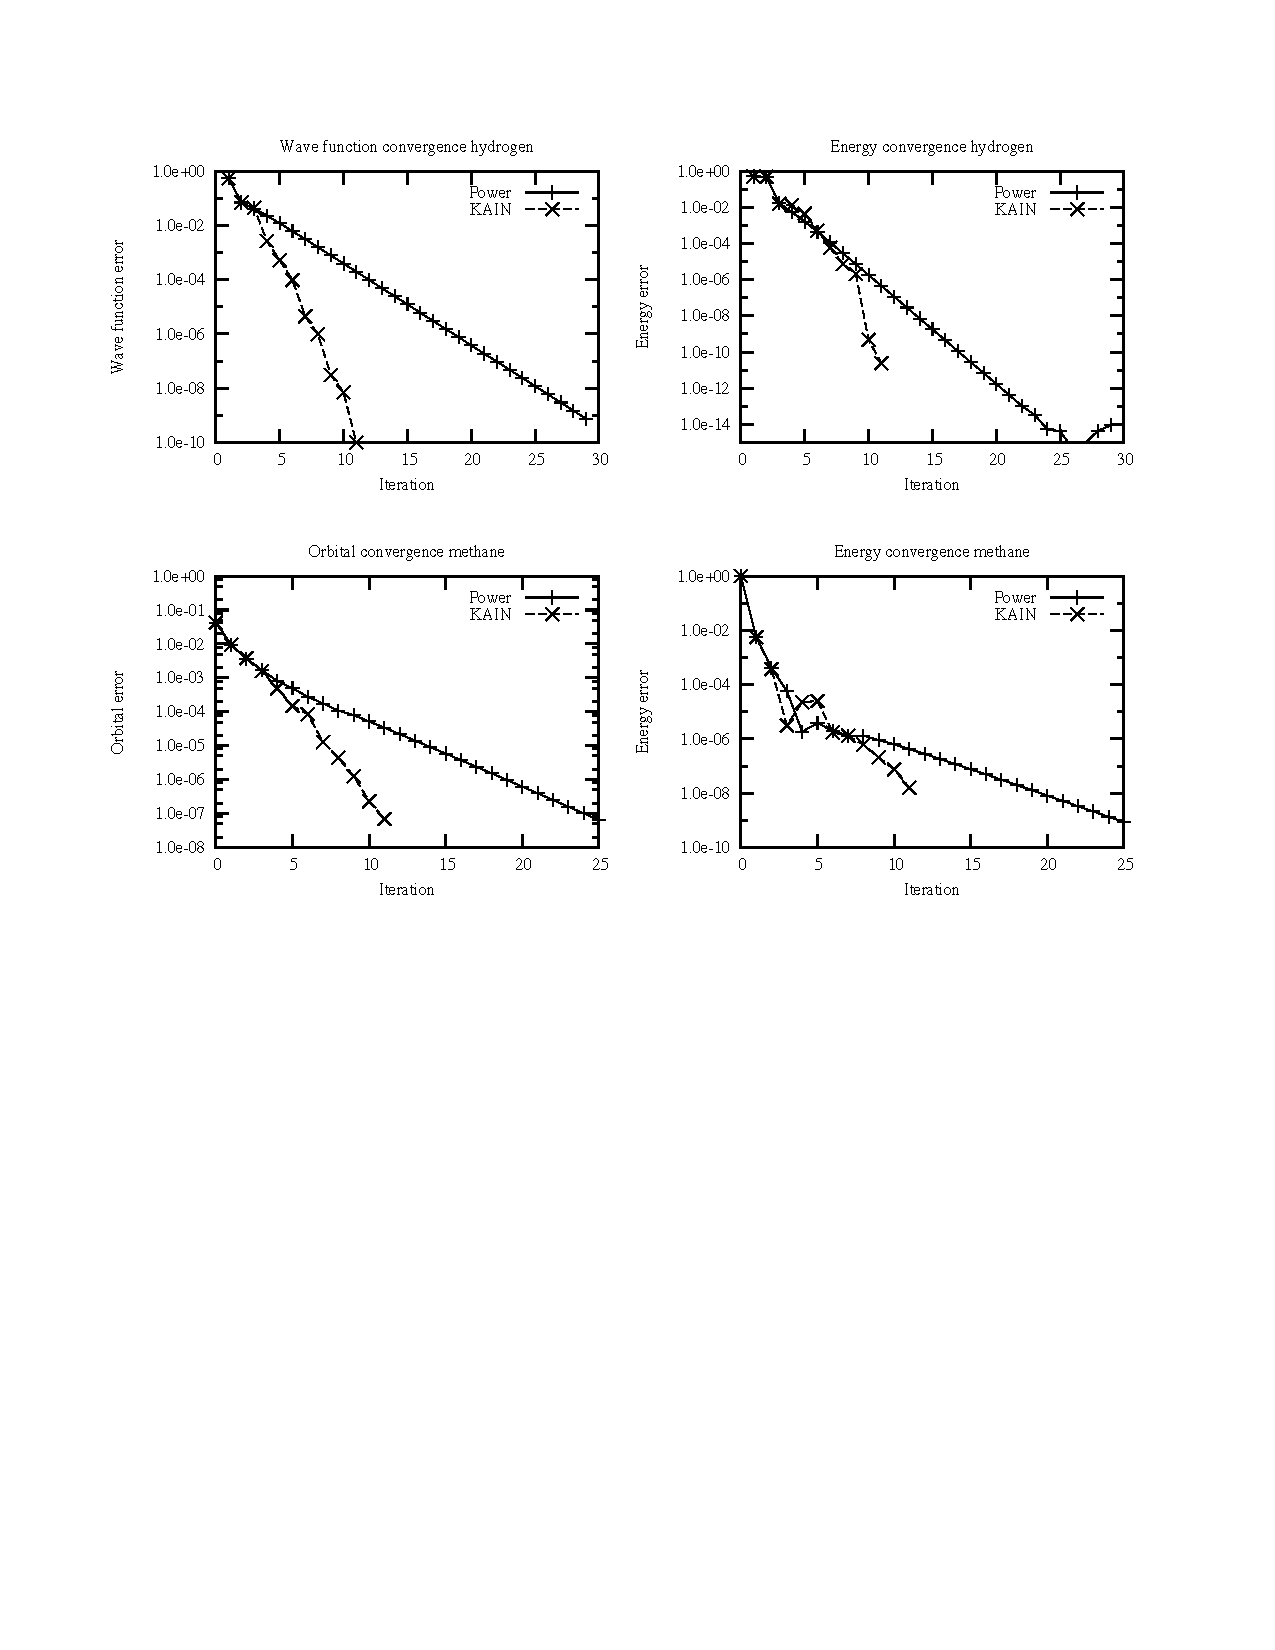
\includegraphics[scale=0.3, clip, viewport = 0 0 900 280]{figures/convergence.pdf}
    \end{center}
    }
    \only<2>{
    \begin{center}
    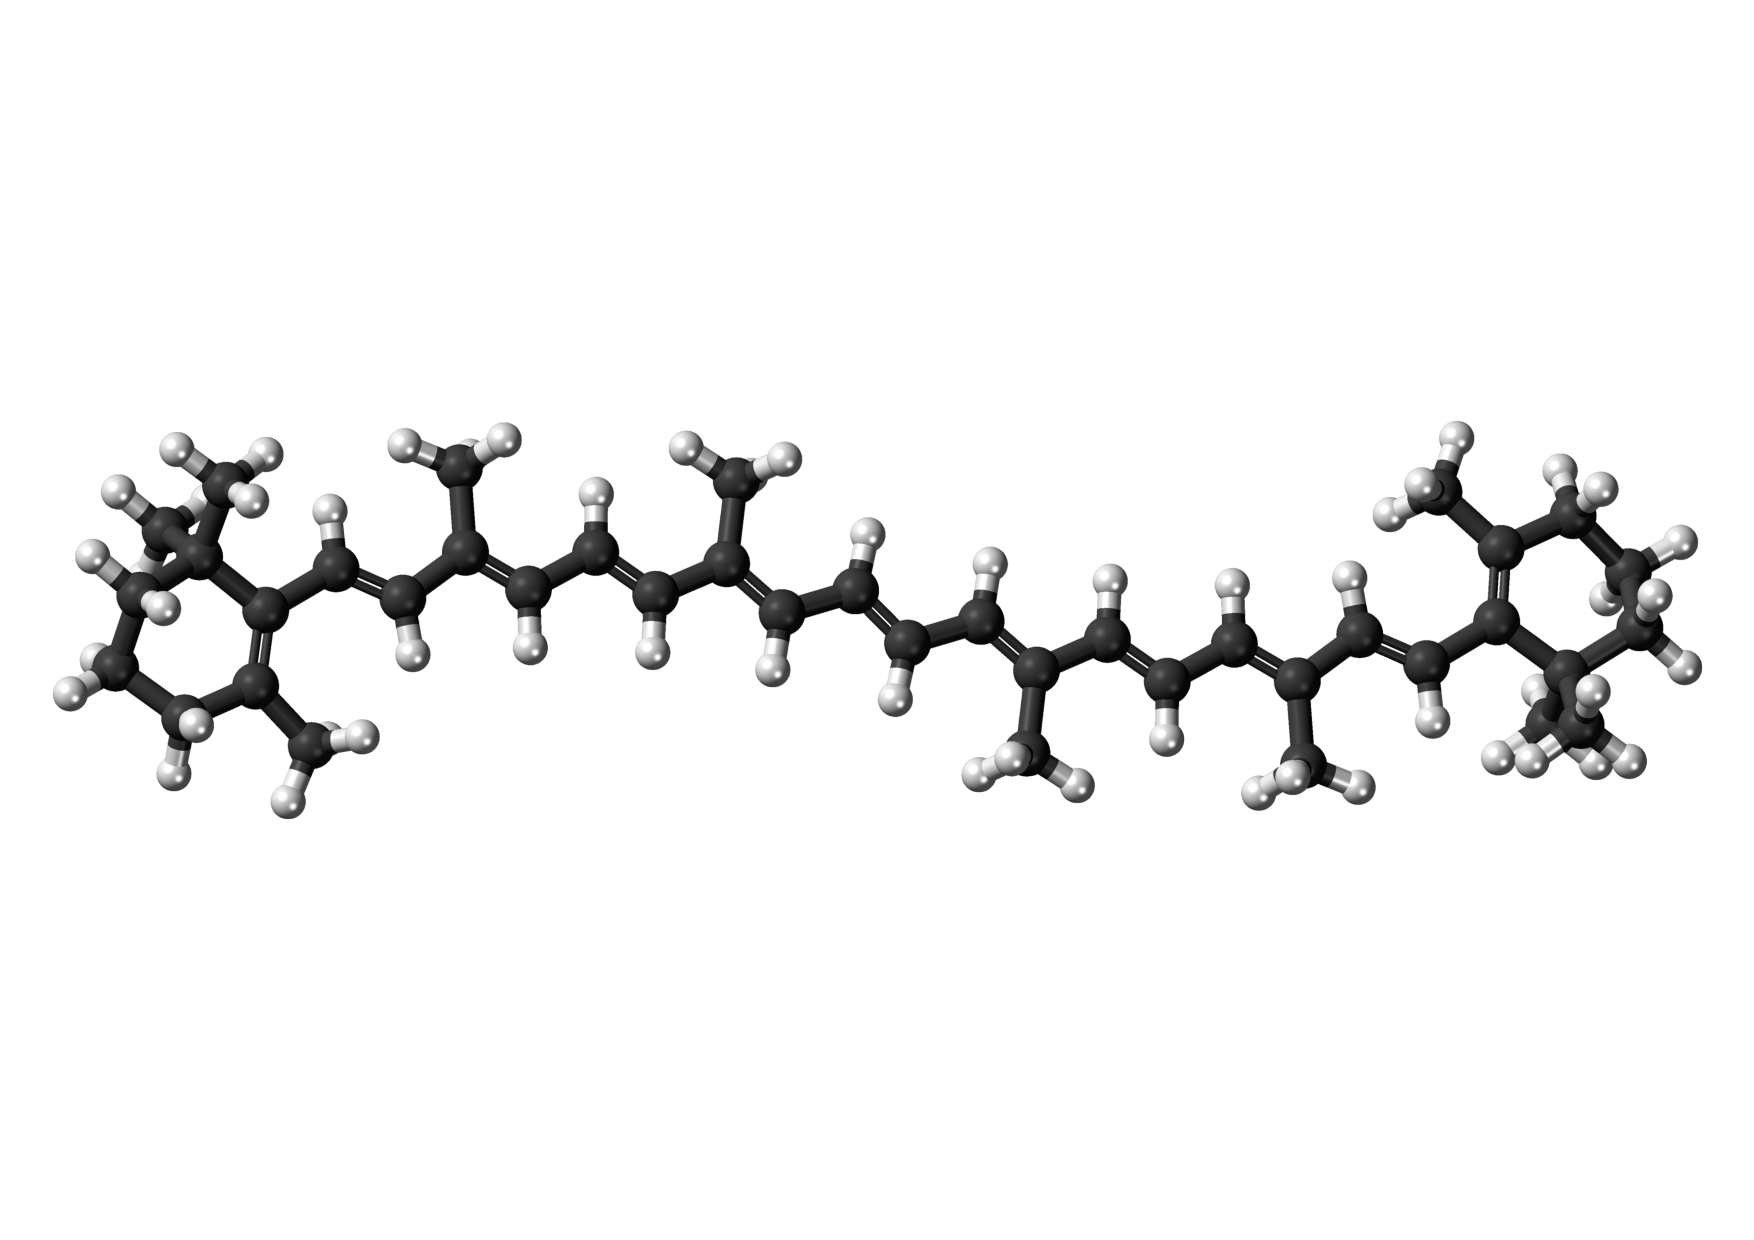
\includegraphics[scale=0.3, clip, viewport = 0 150 900 430]{figures/beta-carotene.pdf}
    \end{center}
    }
\end{frame}

\begin{frame}
    \frametitle{Density Functional Theory}
    \centering
    \textbf{Dramatically reduce the dimensionality}
    \begin{equation}
	\nonumber
	\rho(\boldsymbol{r}_1) = N \int |\Psi(\boldsymbol{r}_1, \boldsymbol{r}_2,\dots,
	\boldsymbol{r}_N)|^2 d\boldsymbol{r}_2\cdots d\boldsymbol{r}_N
    \end{equation}

    \vspace{8mm}

    \centering
    \textbf{Universal energy functional}
    \begin{equation}
	\nonumber
	E[\rho] = T[\rho] + V_{ne}[\rho] + V_{ee}[\rho]
    \end{equation}

    \vspace{10mm}

    \begin{columns}
    \begin{column}{.35\textwidth}
    \centering
    \textbf{Kinetic energy}
    \begin{align}
	\nonumber
	T[\rho]         &= ?
    \end{align}
    \end{column}
    \begin{column}{.30\textwidth}
    \centering
    \textbf{Nuclear-Electron}
    \begin{align}
	\nonumber
	V_{ne}[\rho]	&= \int \rho(r)v_{nuc}(r)\ud r
    \end{align}
    \end{column}
    \begin{column}{.35\textwidth}
    \centering
    \textbf{Electron-Electron}
    \begin{align}
	\nonumber
	V_{ee}[\rho]    &= ?
    \end{align}
    \end{column}
    \end{columns}    
\end{frame}

\begin{frame}
    \frametitle{Kohn-Sham DFT}
    \centering
    \textbf{Introduce one-electron orbitals}
    \begin{equation}
	\nonumber
	\rho(r) = \sum_i |\orbital_i(r)|^2
    \end{equation}

    \vspace{5mm}

    \begin{columns}
    \begin{column}{.50\textwidth}
    \centering
    \textbf{Non-interacting kinetic energy}
    \begin{equation}
	\nonumber
	T[\rho] \approx T_s[\rho] = \sum_i \bra{\orbital_i}-\frac{1}{2}\nabla^2\ket{\orbital_i}
    \end{equation}
    \end{column}
    \begin{column}{.50\textwidth}
    \centering
    \textbf{Classical Coulomb repulsion}
    \begin{equation}
	\nonumber
	V_{ee}[\rho] \approx J[\rho] = \frac{1}{2} \int \rho(r)v_{el}(r)\ud r
    \end{equation}
    \end{column}
    \end{columns}

    \vspace{8mm}

    \textbf{Exchange-Correlation energy}
    \begin{equation}
	\nonumber
	E_{xc}[\rho] = \Big(T[\rho] - T_s[\rho]\Big) + \Big(V_{ee}[\rho] - J[\rho]\Big)
    \end{equation}

    \vspace{5mm}

    \textbf{Kohn-Sham energy expression}
    \begin{equation}
	\nonumber
	E[\rho] = T_s[\rho] + V_{ne}[\rho] + J[\rho] + E_{xc}[\rho]
    \end{equation}
\end{frame}

%\begin{frame}
%    \frametitle{Variation principle}
%    \centering
%    \textbf{leads to the Euler equation}
%    \begin{equation}
%        \nonumber
%        \frac{\delta T_s}{\delta\rho} +
%        \frac{\delta V_{en}}{\delta\rho} +
%        \frac{\delta J}{\delta\rho} +
%        \frac{\delta E_{xc}}{\delta\rho}
%        = \mu 
%    \end{equation}
%    \textbf{chemical potential $\mu$ is a Lagrange multiplier that fixes the number of
%    electrons}
%\end{frame}

\begin{frame}
    \frametitle{Kohn-Sham DFT}
    \centering
    \begin{columns}
    \begin{column}{.50\textwidth}
    \centering
    \textbf{Energy expressions}
    \begin{align}
	\nonumber
	V_{ne}[\rho]	&= \int \rho(r)v_{nuc}(r)\ud r\\
	\nonumber
			&\\
	\nonumber
	J[\rho] &= \frac{1}{2} \int \rho(r)v_{el}(r)\ud r\\
	\nonumber
			&\\
	\nonumber
	E_{xc}[\rho]	&= \int F_{xc}(\rho, \nabla\rho, \dots) \ud r
    \end{align}
    \end{column}
    \begin{column}{.50\textwidth}
    \centering
    \textbf{Potentials}
    \begin{align}
	\nonumber
        %\frac{\delta V_{en}}{\delta\rho} &=
	v_{nuc}(r) &=
        -\sum_I\frac{Z_I}{|r-R_I|}\\
	\nonumber
			&\\
	\nonumber
        %\frac{\delta J}{\delta\rho} &=
	v_{el}(r) &=
	\int \frac{\rho(r')}{4\pi|r-r'|} \ud r'\\
	\nonumber
			&\\
	\nonumber
        %\frac{\delta E_{xc}}{\delta\rho} &=
	v_{xc}(r) &=
        \frac{\partial F_{xc}}{\partial \rho} - \nabla \cdot \frac{\partial
        F_{xc}}{\partial \nabla \rho}
    \end{align}
    \end{column}
    \end{columns}    

    \vspace{5mm}

    \centering
    \textbf{Kohn-Sham potential}
    \begin{equation}
        \nonumber
        v_{eff}(r) = v_{nuc}(r) + v_{el}(r) + v_{xc}(r)
    \end{equation}

%    \textbf{Minimizing the energy}
%    \begin{equation}
%        E_0 = \mymin{\rho}\ E[\rho]
%    \end{equation}

    \vspace{5mm}

    \centering
    \textbf{Kohn-Sham equations}
    \begin{equation}
	\nonumber
	\bigg[-\frac{1}{2}\nabla^2 + v_{eff}(r)\bigg]\orbital_i(r) = \epsilon_i \orbital_i(r)
    \end{equation}

\end{frame}

\begin{frame}
    \frametitle{Basis sets}
    \begin{columns}
    \begin{column}{.10\textwidth}
    \end{column}
    \begin{column}{.30\textwidth}
    \textbf{Attractive features}
    \begin{itemize}
        \item {\color{green} Accuracy}
        \item {\color{green} Compactness}
        \item {\color{red} Efficiency}
        \item {\color{yellow} Systematicity}
        \item {\color{red} Universality}
    \end{itemize}
    \end{column}
    \begin{column}{.60\textwidth}
    \centering
    \textbf{Atoms-centered basis sets}
    \begin{equation}
        \nonumber
        \chi(\rvec) = R(r)Y_{lm}(\theta,\varphi)
    \end{equation}
    
    \vspace{5mm}

    \textbf{Slater-type orbitals}
    \begin{equation}
        \nonumber
        R^{STO}(r) \propto e^{-\zeta r}
    \end{equation}
    \end{column}
    \end{columns}    

    \vspace{5mm}

    \begin{center}
    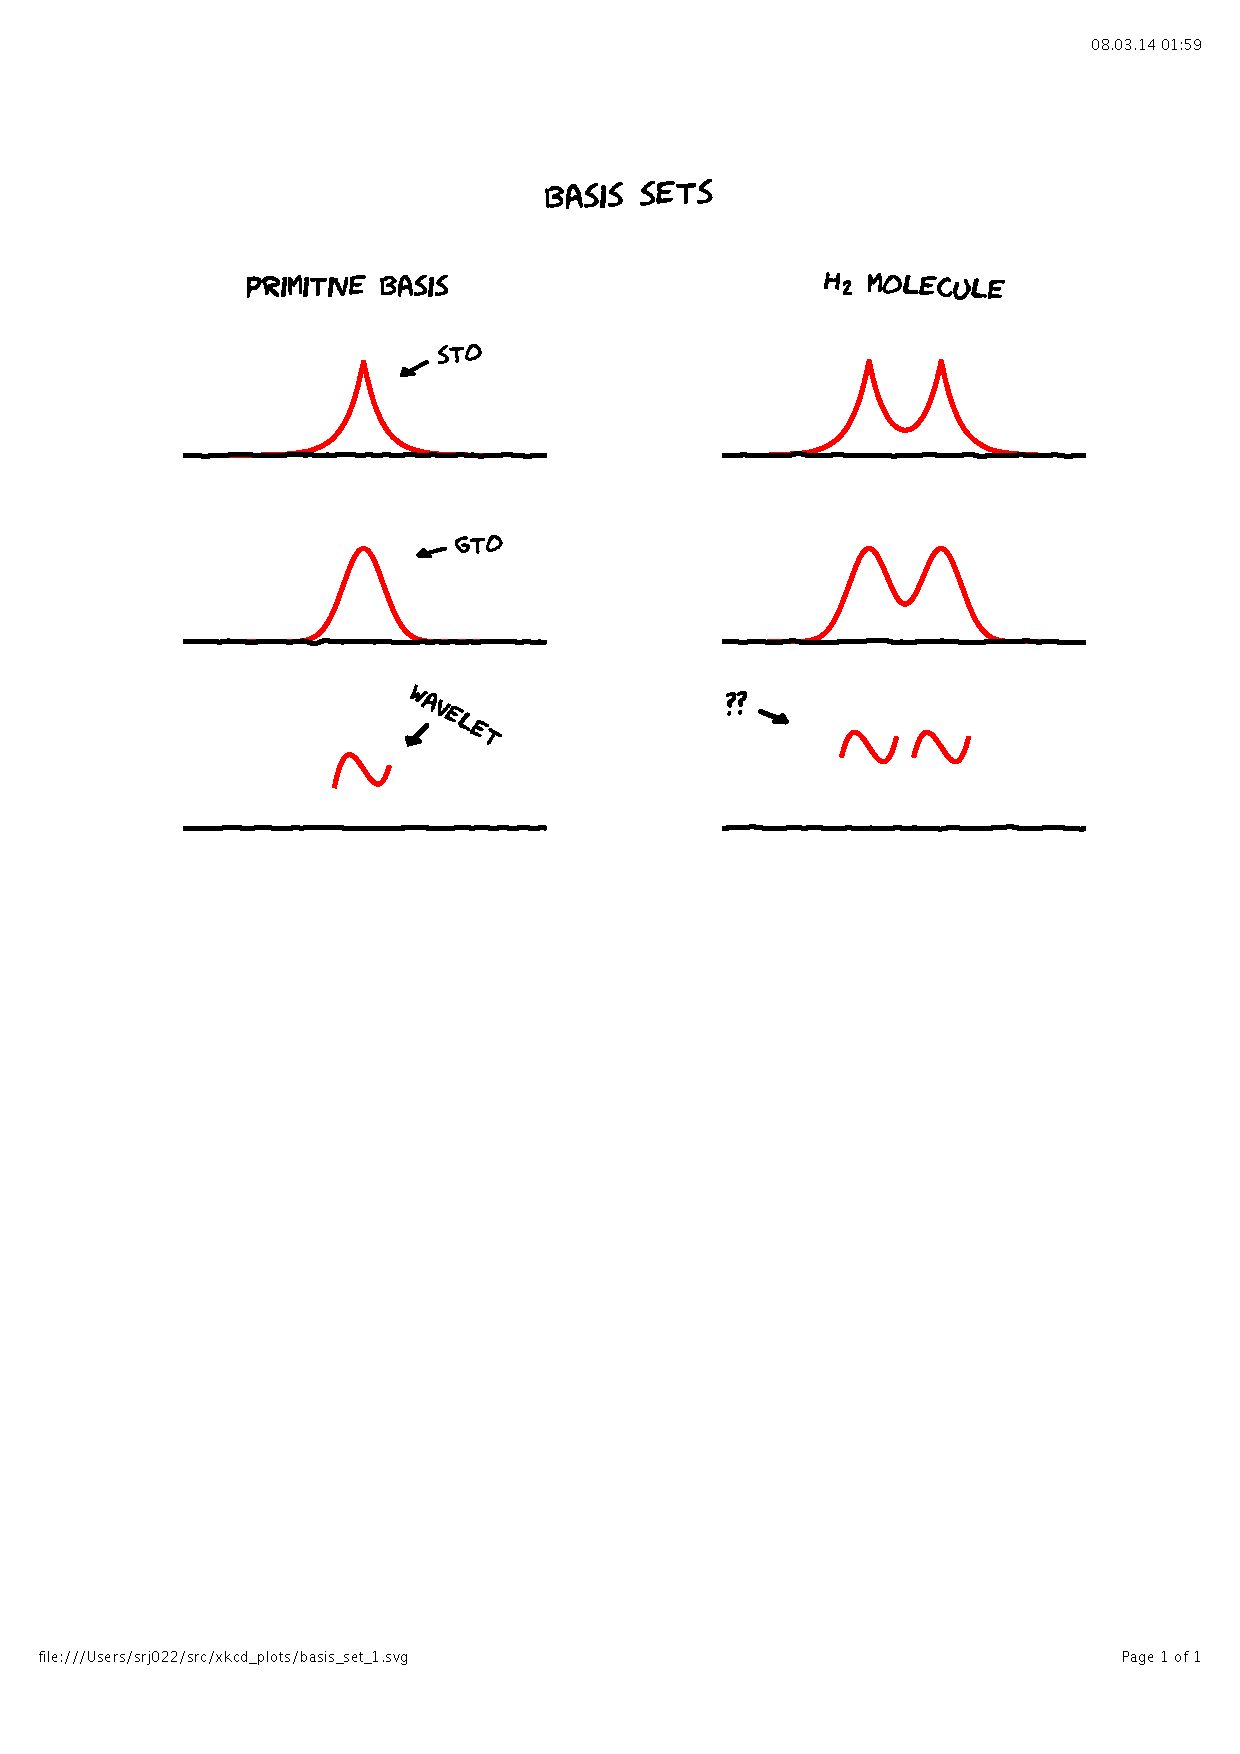
\includegraphics[scale=0.6, clip, viewport = 50 680 550 730]{figures/basis_set_1.pdf}\\
    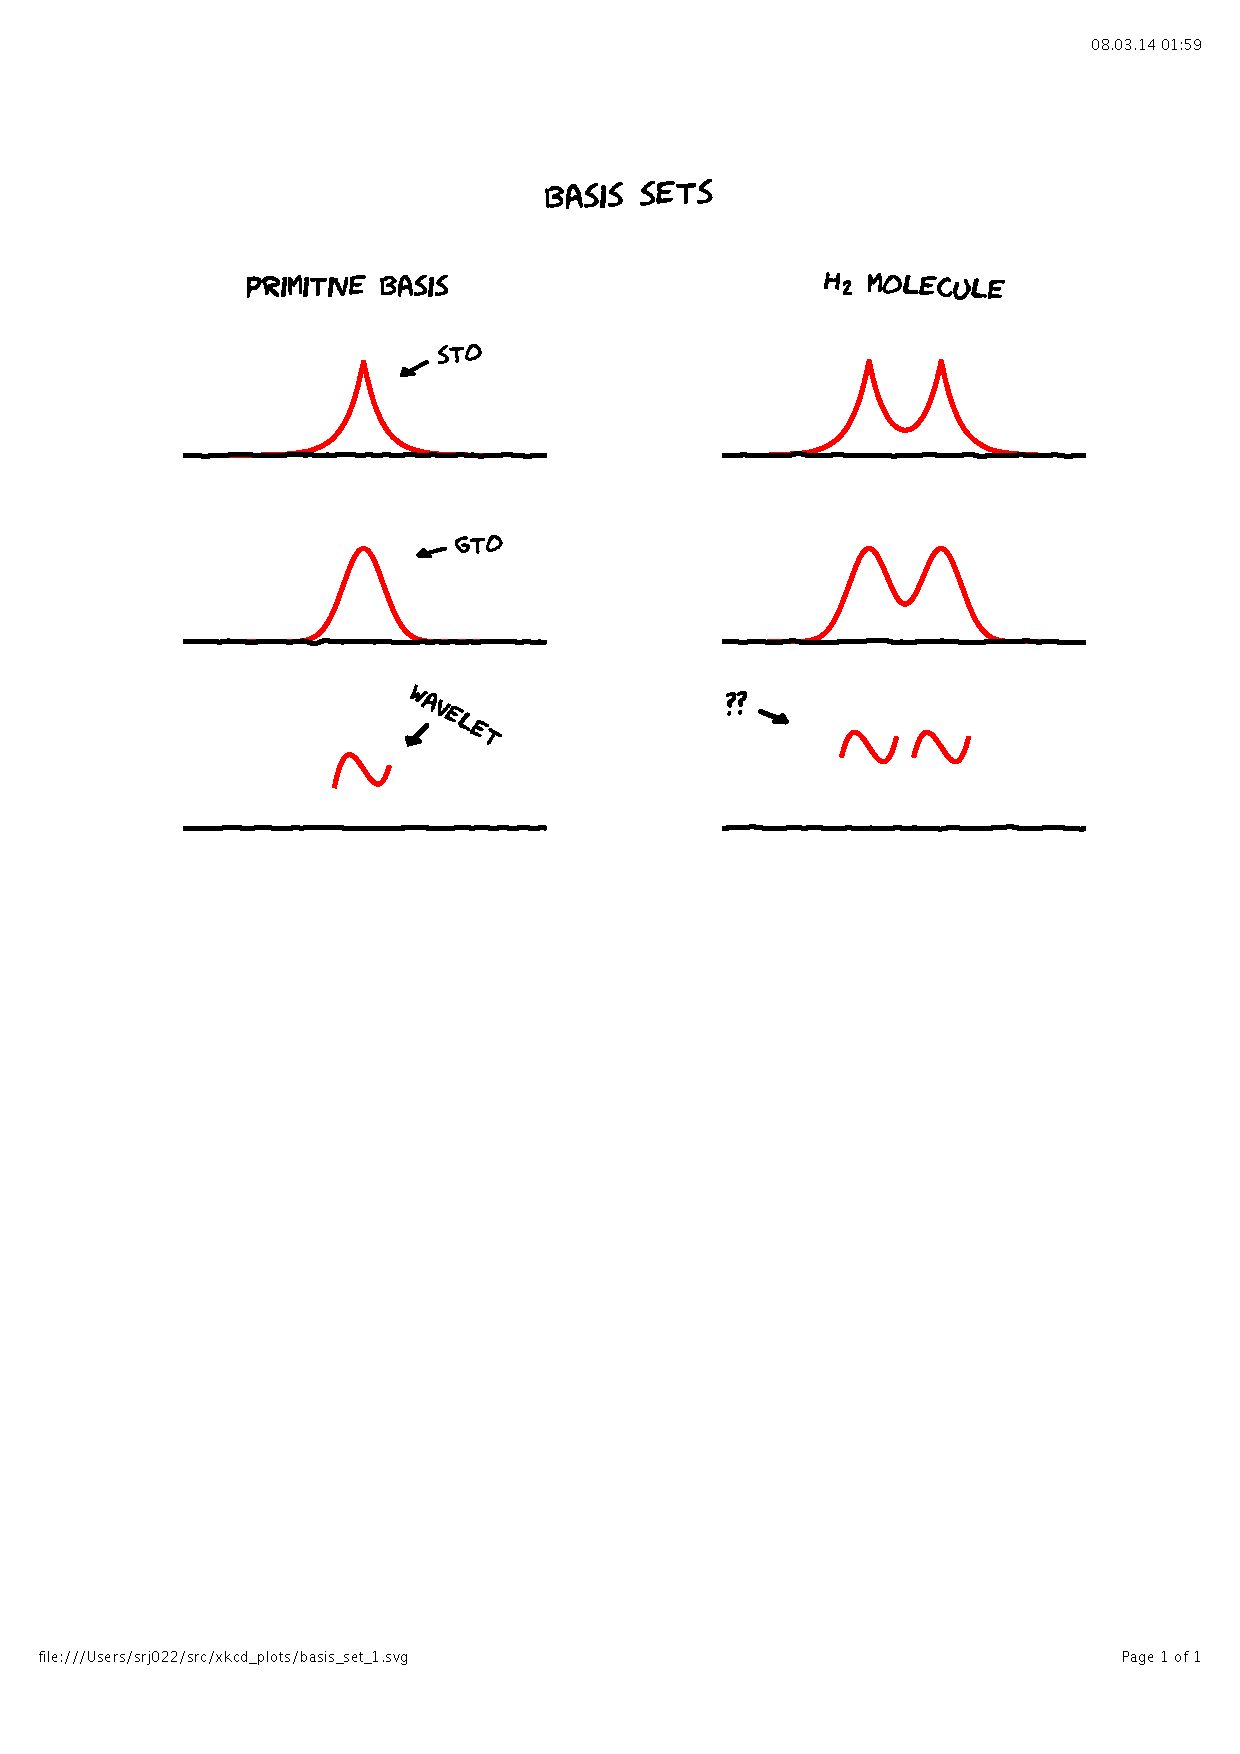
\includegraphics[scale=0.6, clip, viewport = 50 615 550 695]{figures/basis_set_1.pdf}
    \end{center}
\end{frame}

\begin{frame}
    \frametitle{Basis sets}
    \begin{columns}
    \begin{column}{.10\textwidth}
    \end{column}
    \begin{column}{.30\textwidth}
    \textbf{Attractive features}
    \begin{itemize}
        \item {\color{yellow} Accuracy}
        \item {\color{yellow} Compactness}
        \item {\color{green} Efficiency}
        \item {\color{yellow} Systematicity}
        \item {\color{red} Universality}
    \end{itemize}
    \end{column}
    \begin{column}{.60\textwidth}
    \centering
    \textbf{Atoms-centered basis sets}
    \begin{equation}
        \nonumber
        \chi(\rvec) = R(r)Y_{lm}(\theta,\varphi)
    \end{equation}
    
    \vspace{4.2mm}

    \textbf{Gaussian-type orbitals}
    \begin{equation}
        \nonumber
        R^{GTO}(r) \propto e^{-\zeta r^2}
    \end{equation}
    \end{column}
    \end{columns}    

    \vspace{5mm}

    \begin{center}
    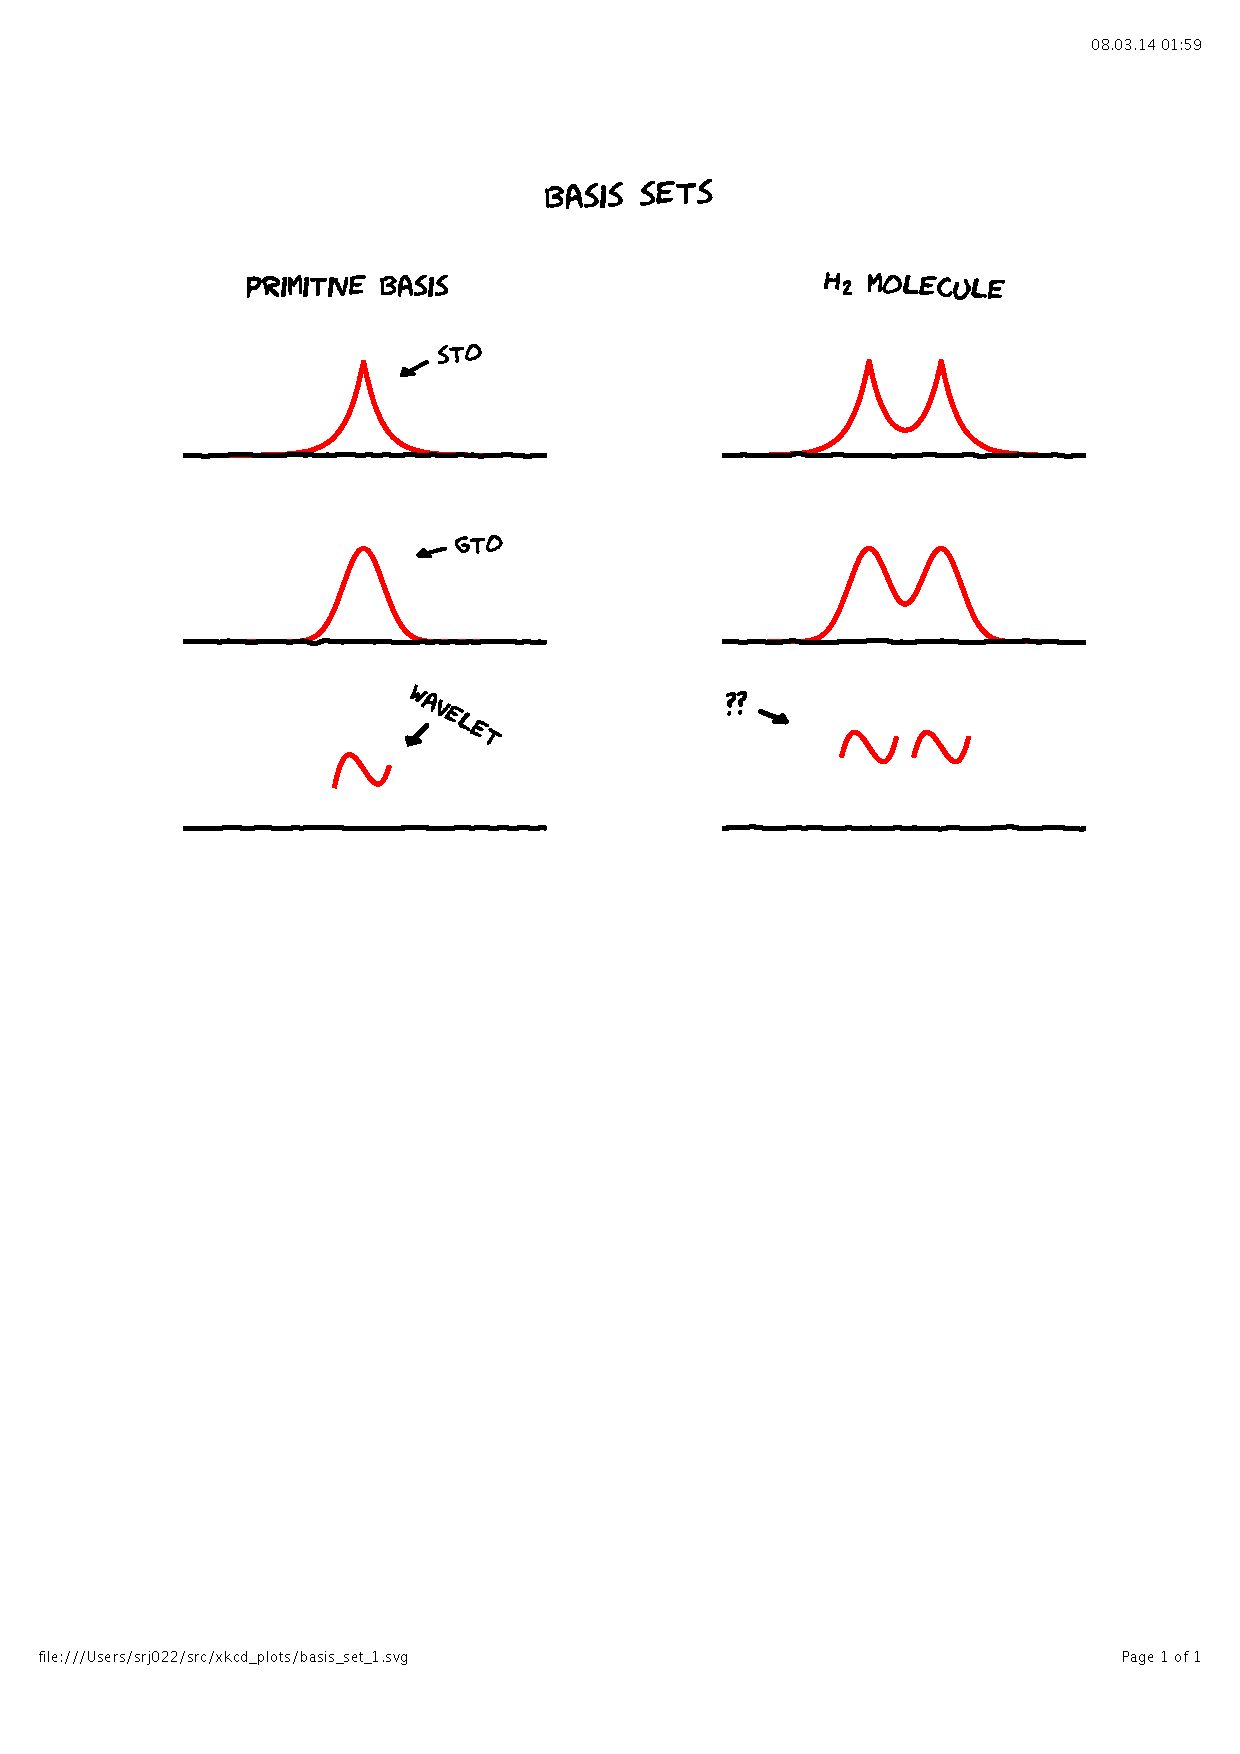
\includegraphics[scale=0.6, clip, viewport = 50 680 550 730]{figures/basis_set_1.pdf}\\
    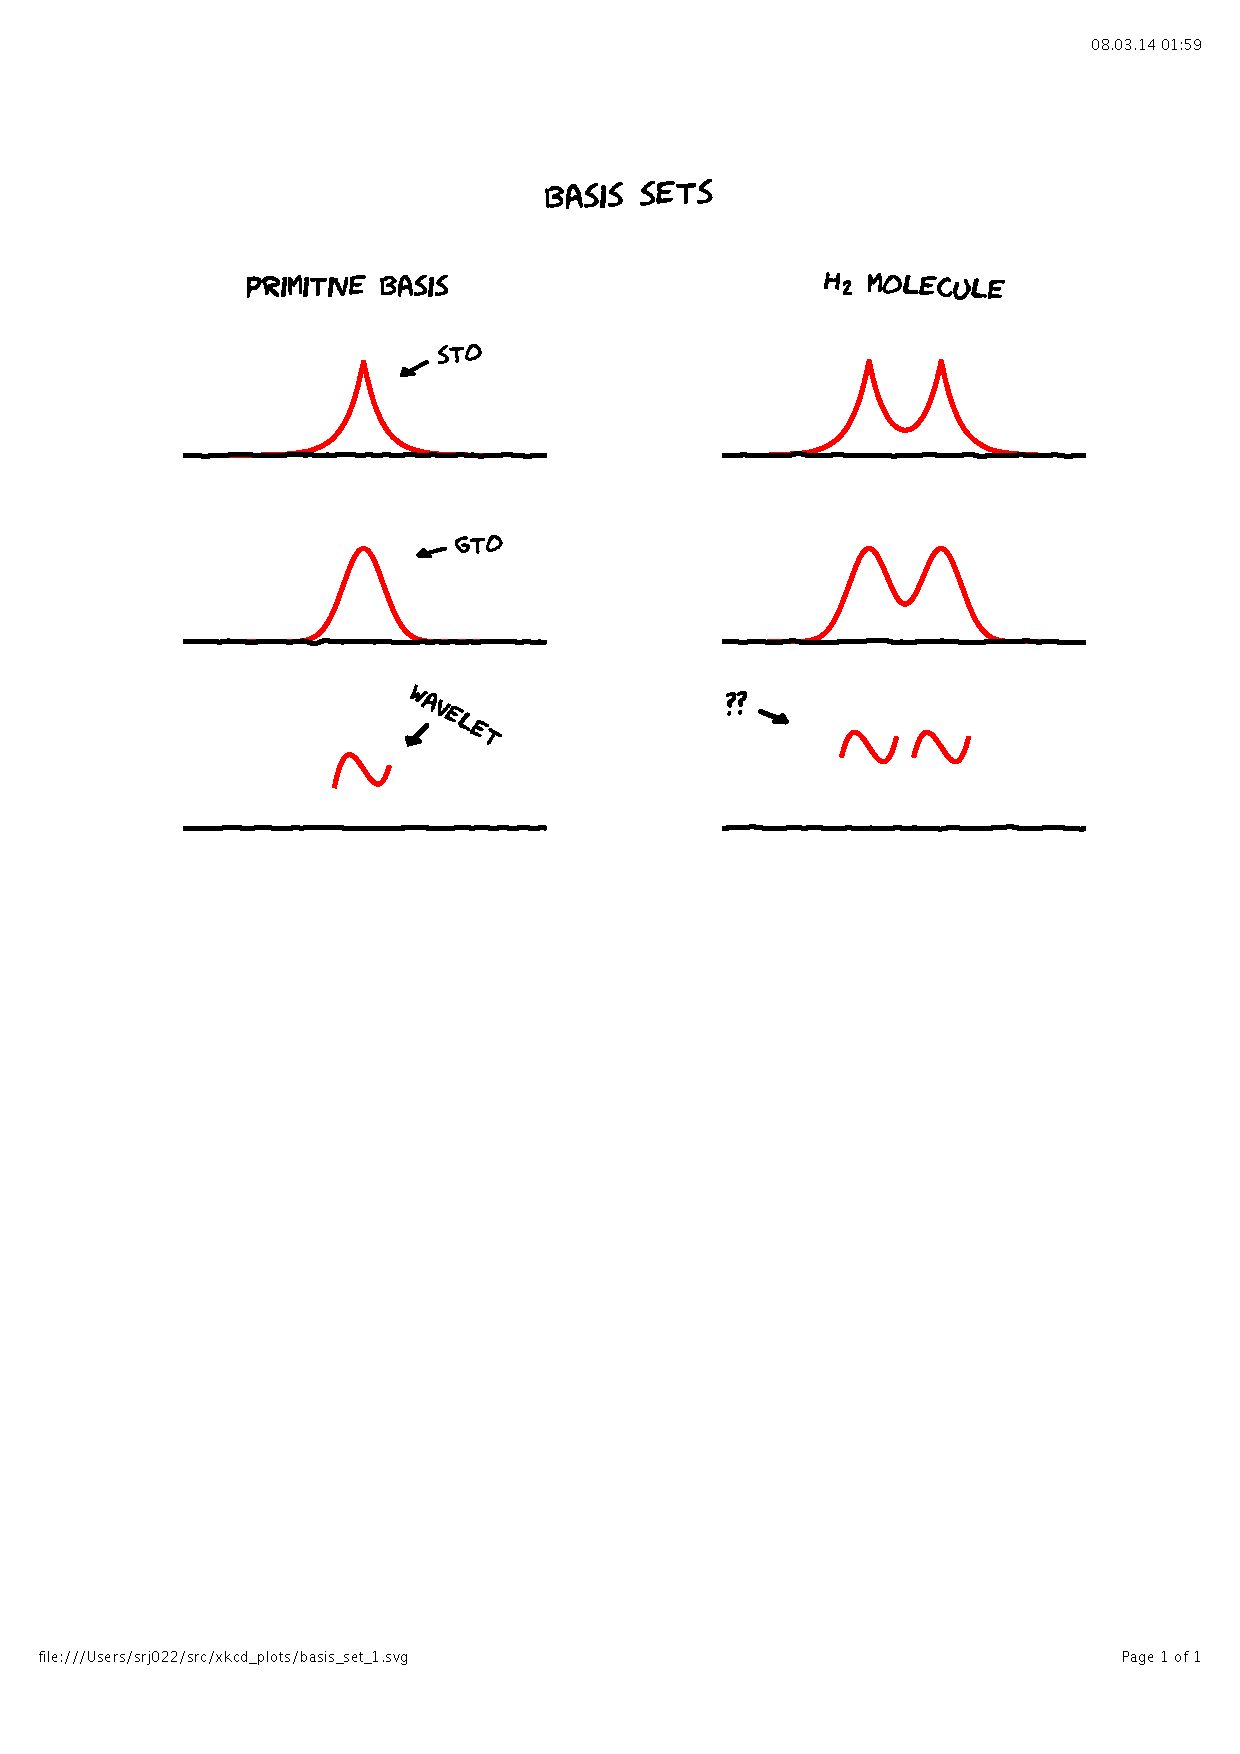
\includegraphics[scale=0.6, clip, viewport = 50 525 550 605]{figures/basis_set_1.pdf}
    \end{center}
\end{frame}

\begin{frame}
    \frametitle{Basis sets}
    \begin{columns}
    \begin{column}{.10\textwidth}
    \end{column}
    \begin{column}{.30\textwidth}
    \textbf{Attractive features}
    \begin{itemize}
        \item {\color{yellow} Accuracy}
        \item {\color{yellow} Compactness}
        \item {\color{green} Efficiency}
        \item {\color{green} Systematicity}
        \item {\color{yellow} Universality}
    \end{itemize}
    \end{column}
    \begin{column}{.60\textwidth}
    \centering
    \textbf{Plane-wave basis sets}
    \begin{equation}
        \nonumber
        \chi(\rvec) = e^{i\bs{k}\cdot\bs{r}}
    \end{equation}
    
    %\vspace{4.2mm}

    %\textbf{Plane waves}
    %\begin{equation}
        %\nonumber
        %\chi(\rvec) = e^{i\bs{k}\cdot\bs{r}}
    %\end{equation}
    \end{column}
    \end{columns}    

    \vspace{5mm}

    \begin{center}
    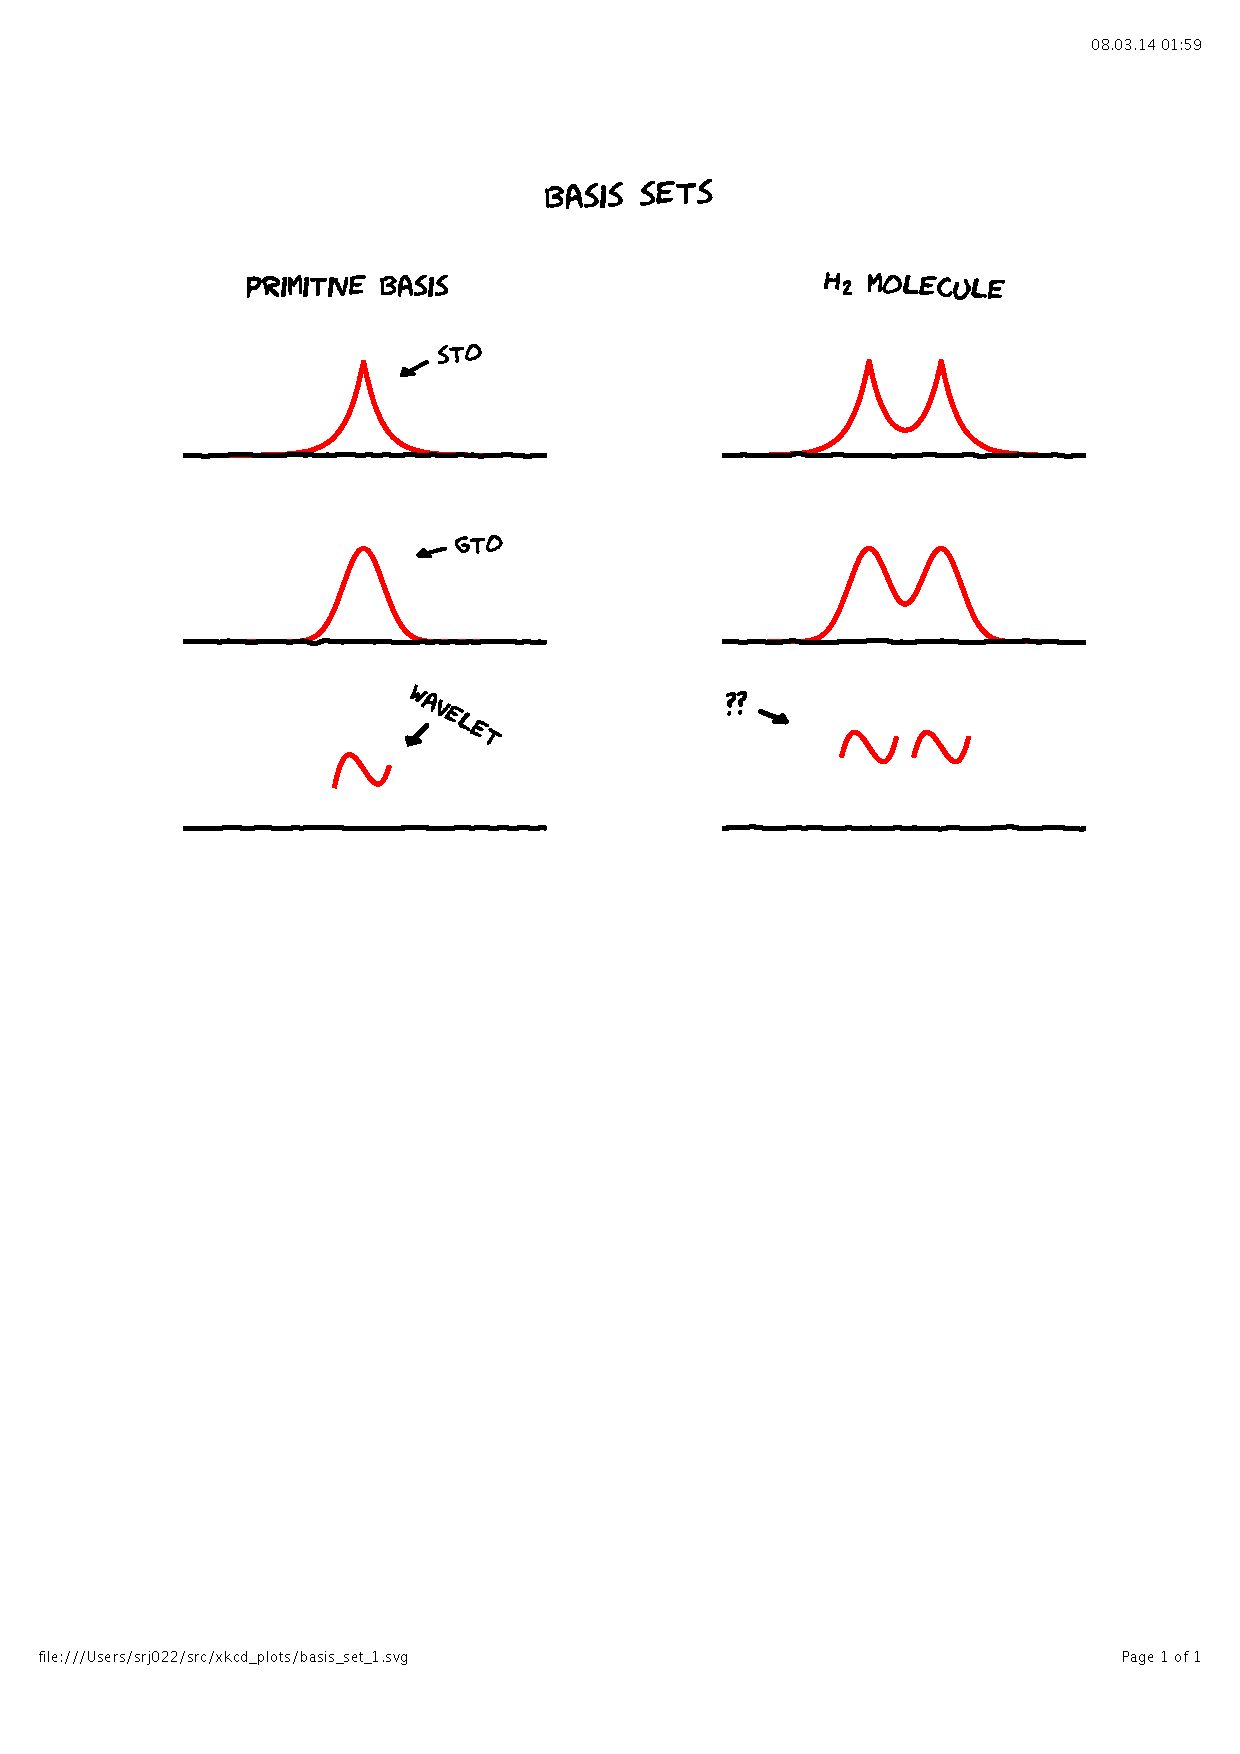
\includegraphics[scale=0.6, clip, viewport = 50 680 550 730]{figures/basis_set_1.pdf}\\
    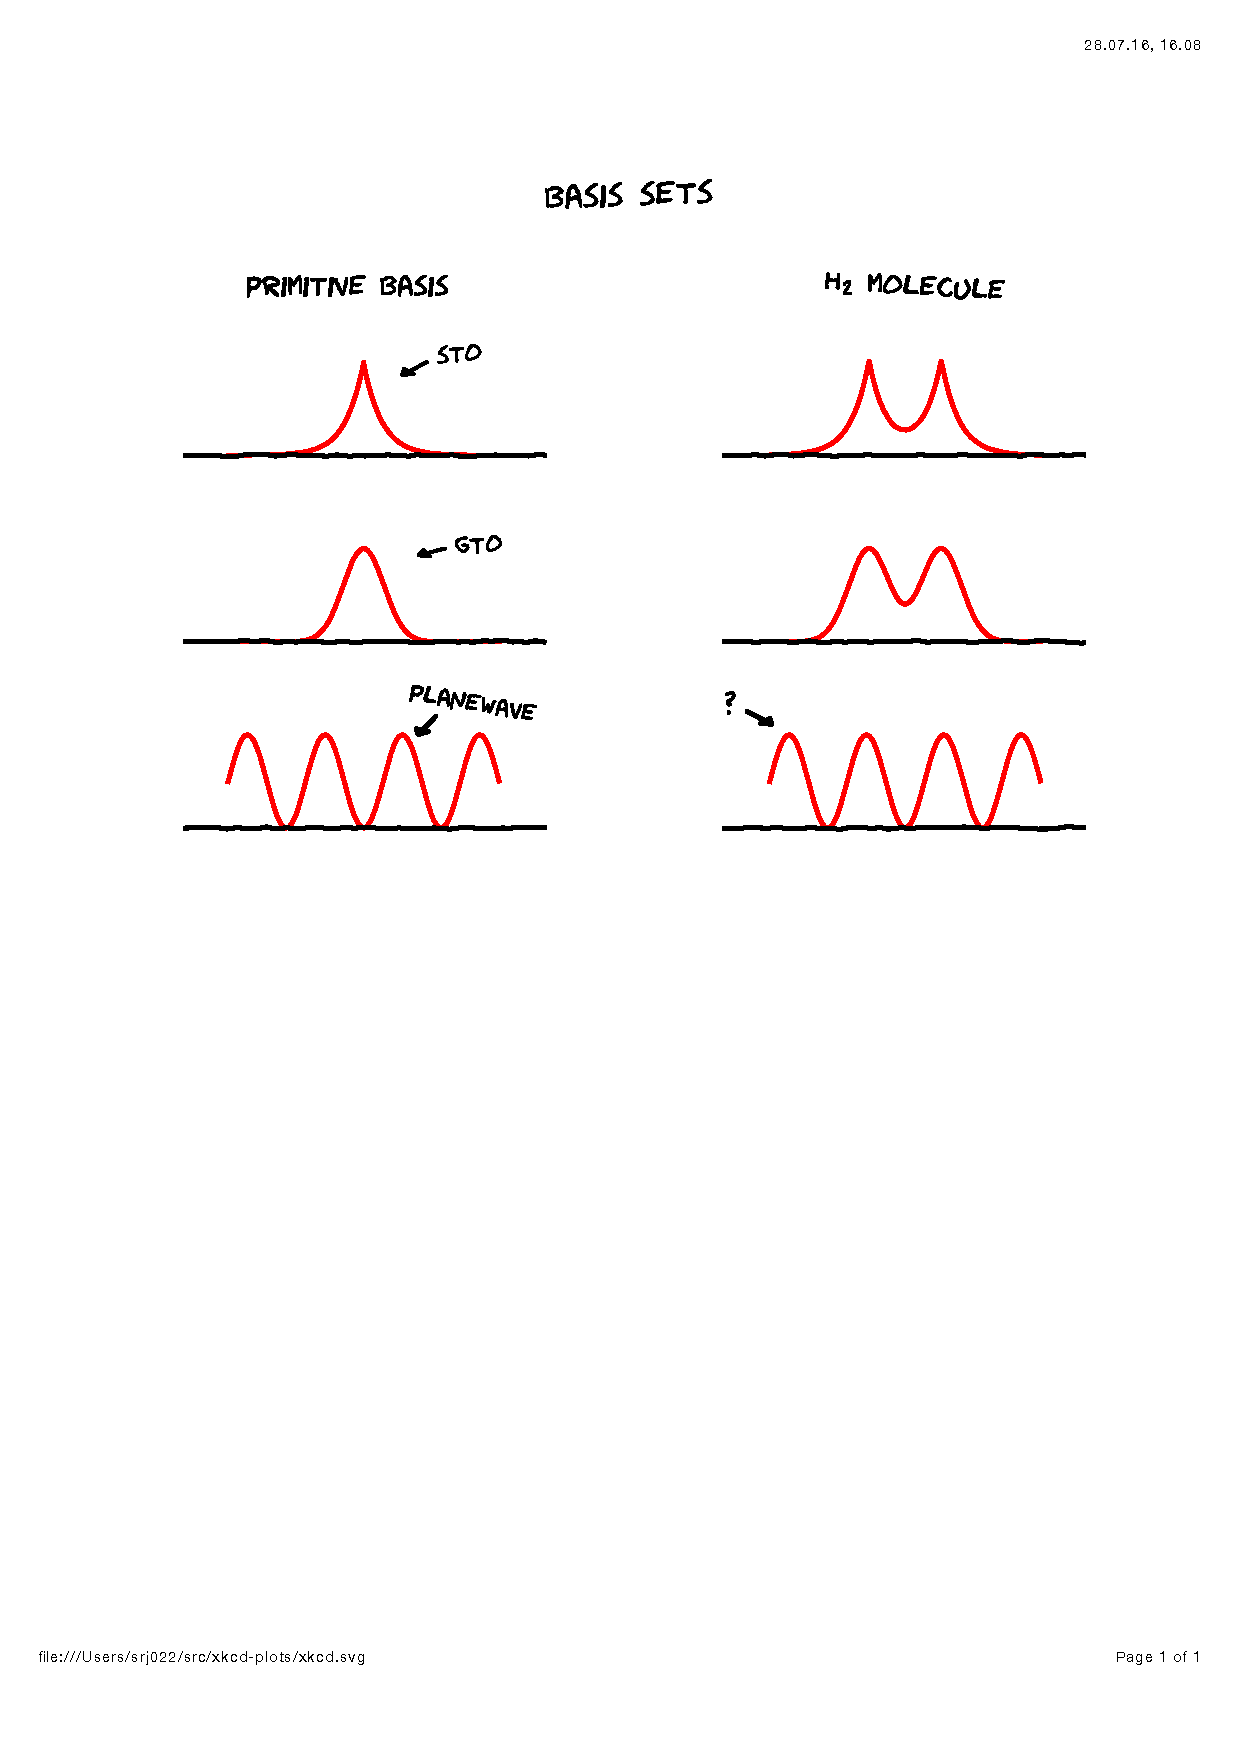
\includegraphics[scale=0.6, clip, viewport = 50 435 550 515]{figures/basis_set_3.pdf}
    \end{center}
\end{frame}


\begin{frame}
    \frametitle{Basis sets}
    \begin{columns}
    \begin{column}{.10\textwidth}
    \end{column}
    \begin{column}{.30\textwidth}
    \textbf{Attractive features}
    \begin{itemize}
        \item {\color{green} Accuracy}
        \item {\color{red} Compactness}
        \item {\color{green} Efficiency}
        \item {\color{green} Systematicity}
        \item {\color{green} Universality}
    \end{itemize}
    \end{column}
    \begin{column}{.60\textwidth}
    \centering
    \textbf{Real-space basis sets}
    \begin{equation}
        \nonumber
        \chi(\rvec) = \phi_i(x)\phi_j(y)\phi_k(z)
    \end{equation}
    
    \vspace{4.2mm}

    \textbf{Multiwavelets}
    \begin{equation}
        \nonumber
        \phi_{j,l}^n(x) = 2^{n/2}\phi_j(2^nx-l)
    \end{equation}
    \end{column}
    \end{columns}    

    \vspace{5mm}

    \begin{center}
    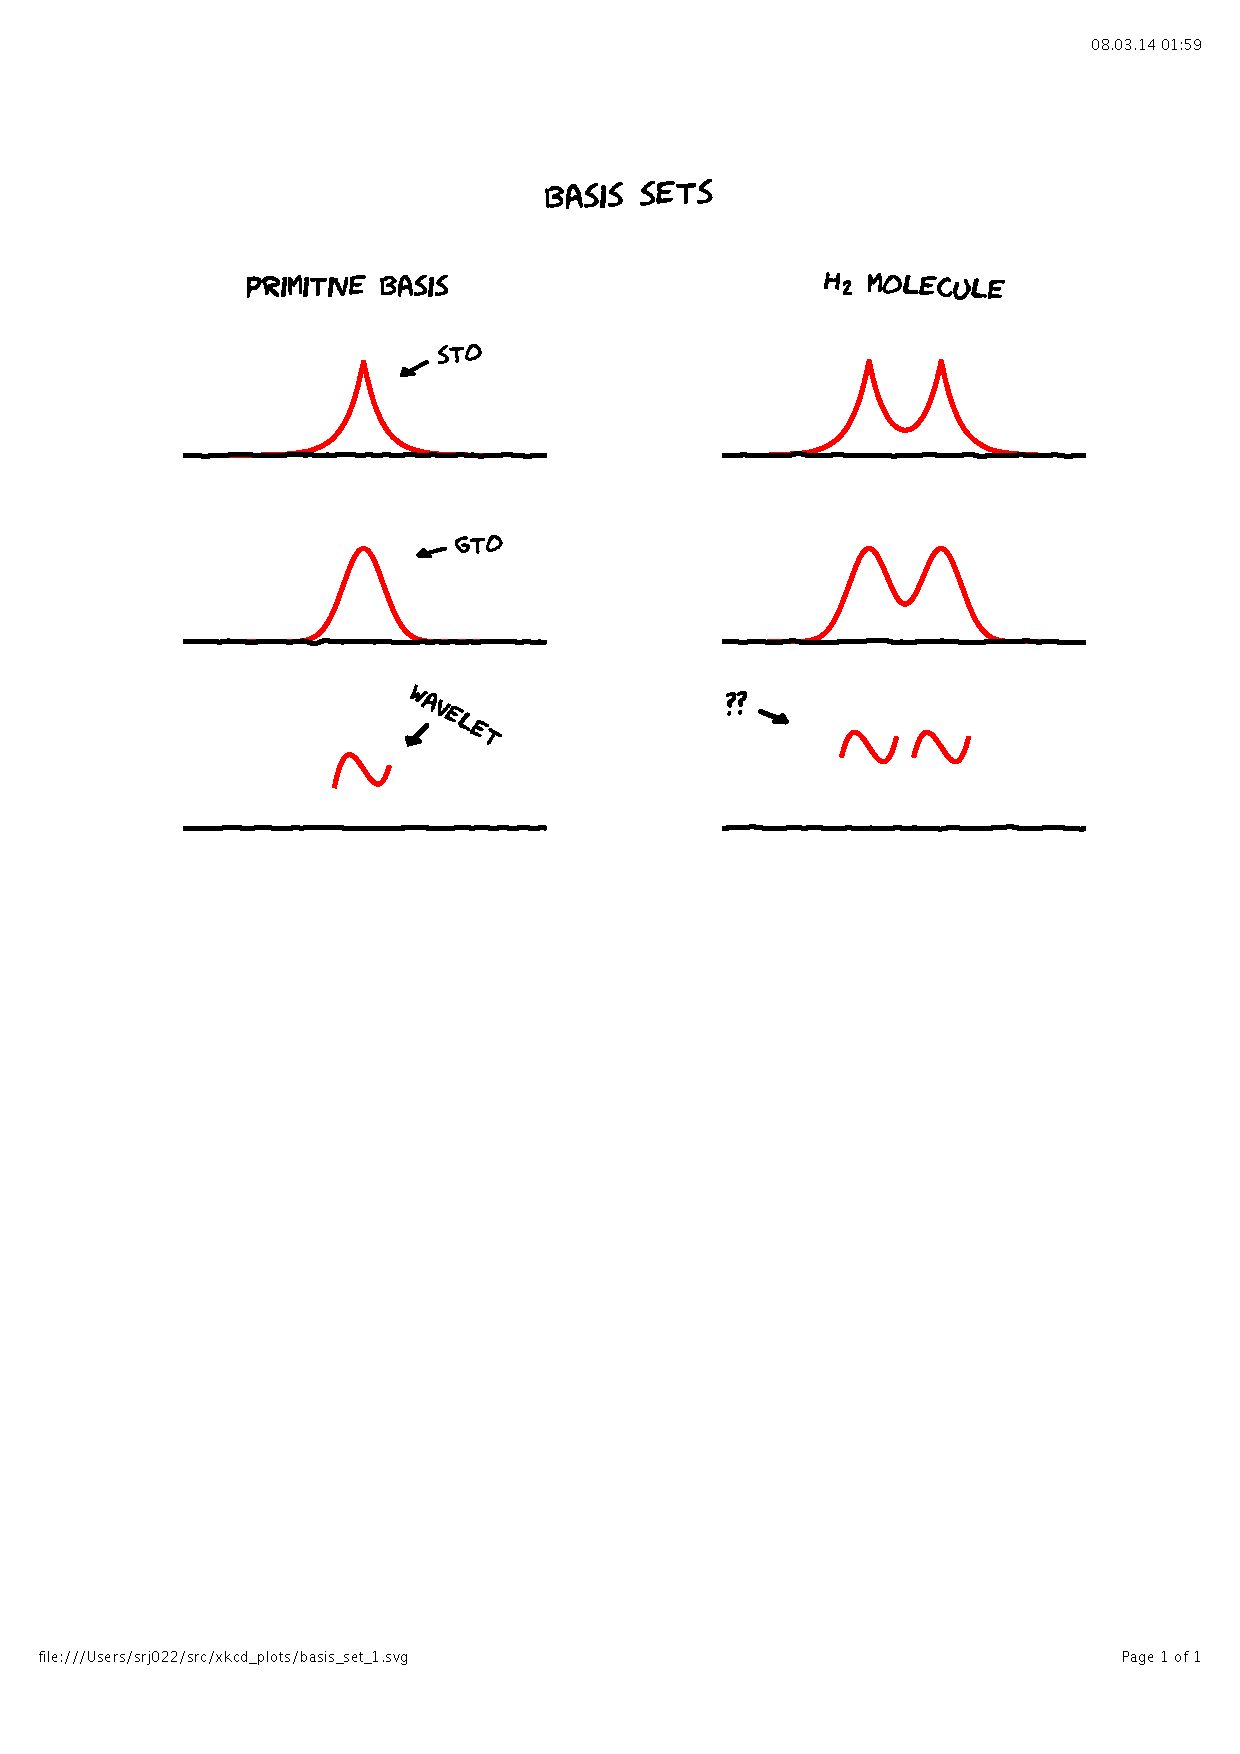
\includegraphics[scale=0.6, clip, viewport = 50 680 550 730]{figures/basis_set_1.pdf}\\
    \only<1>{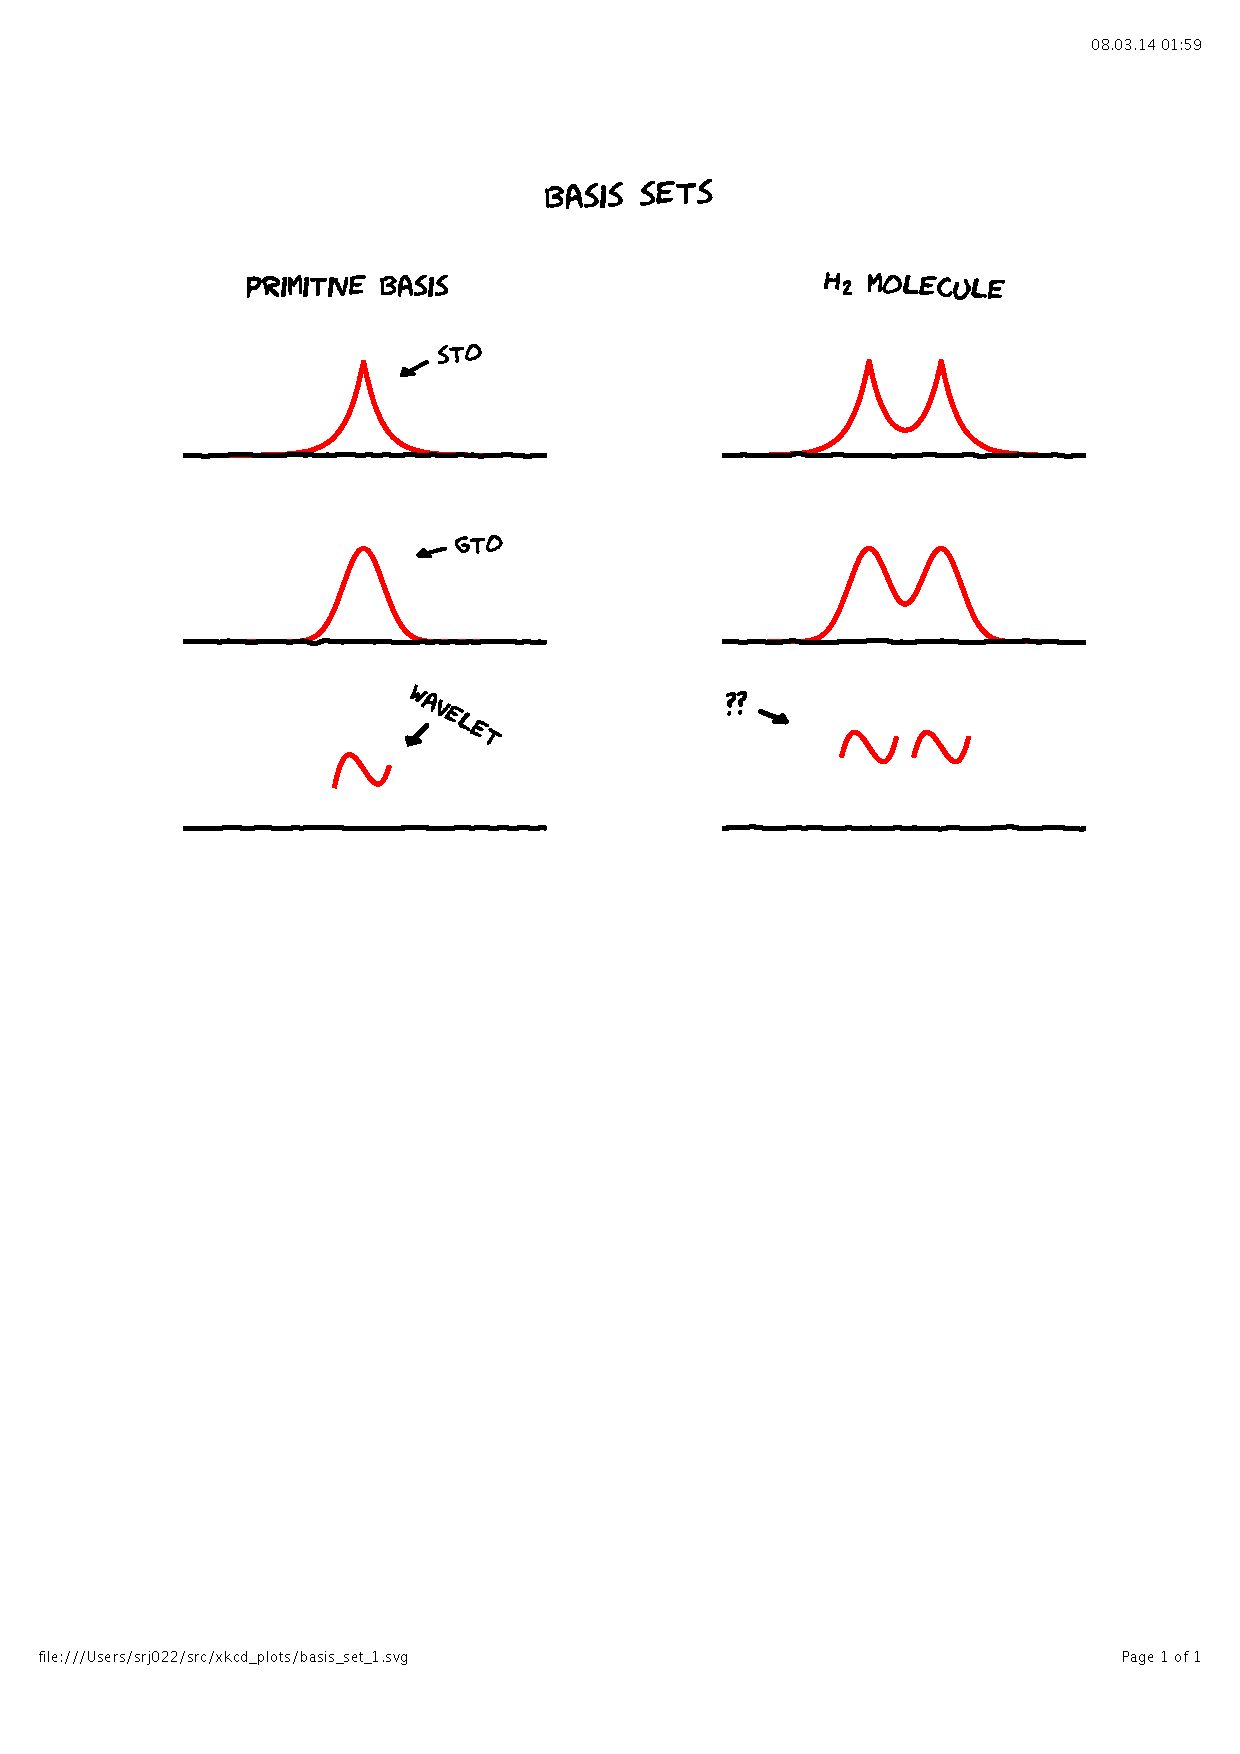
\includegraphics[scale=0.6, clip, viewport = 50 435 550 515]{figures/basis_set_1.pdf}}
    \only<2>{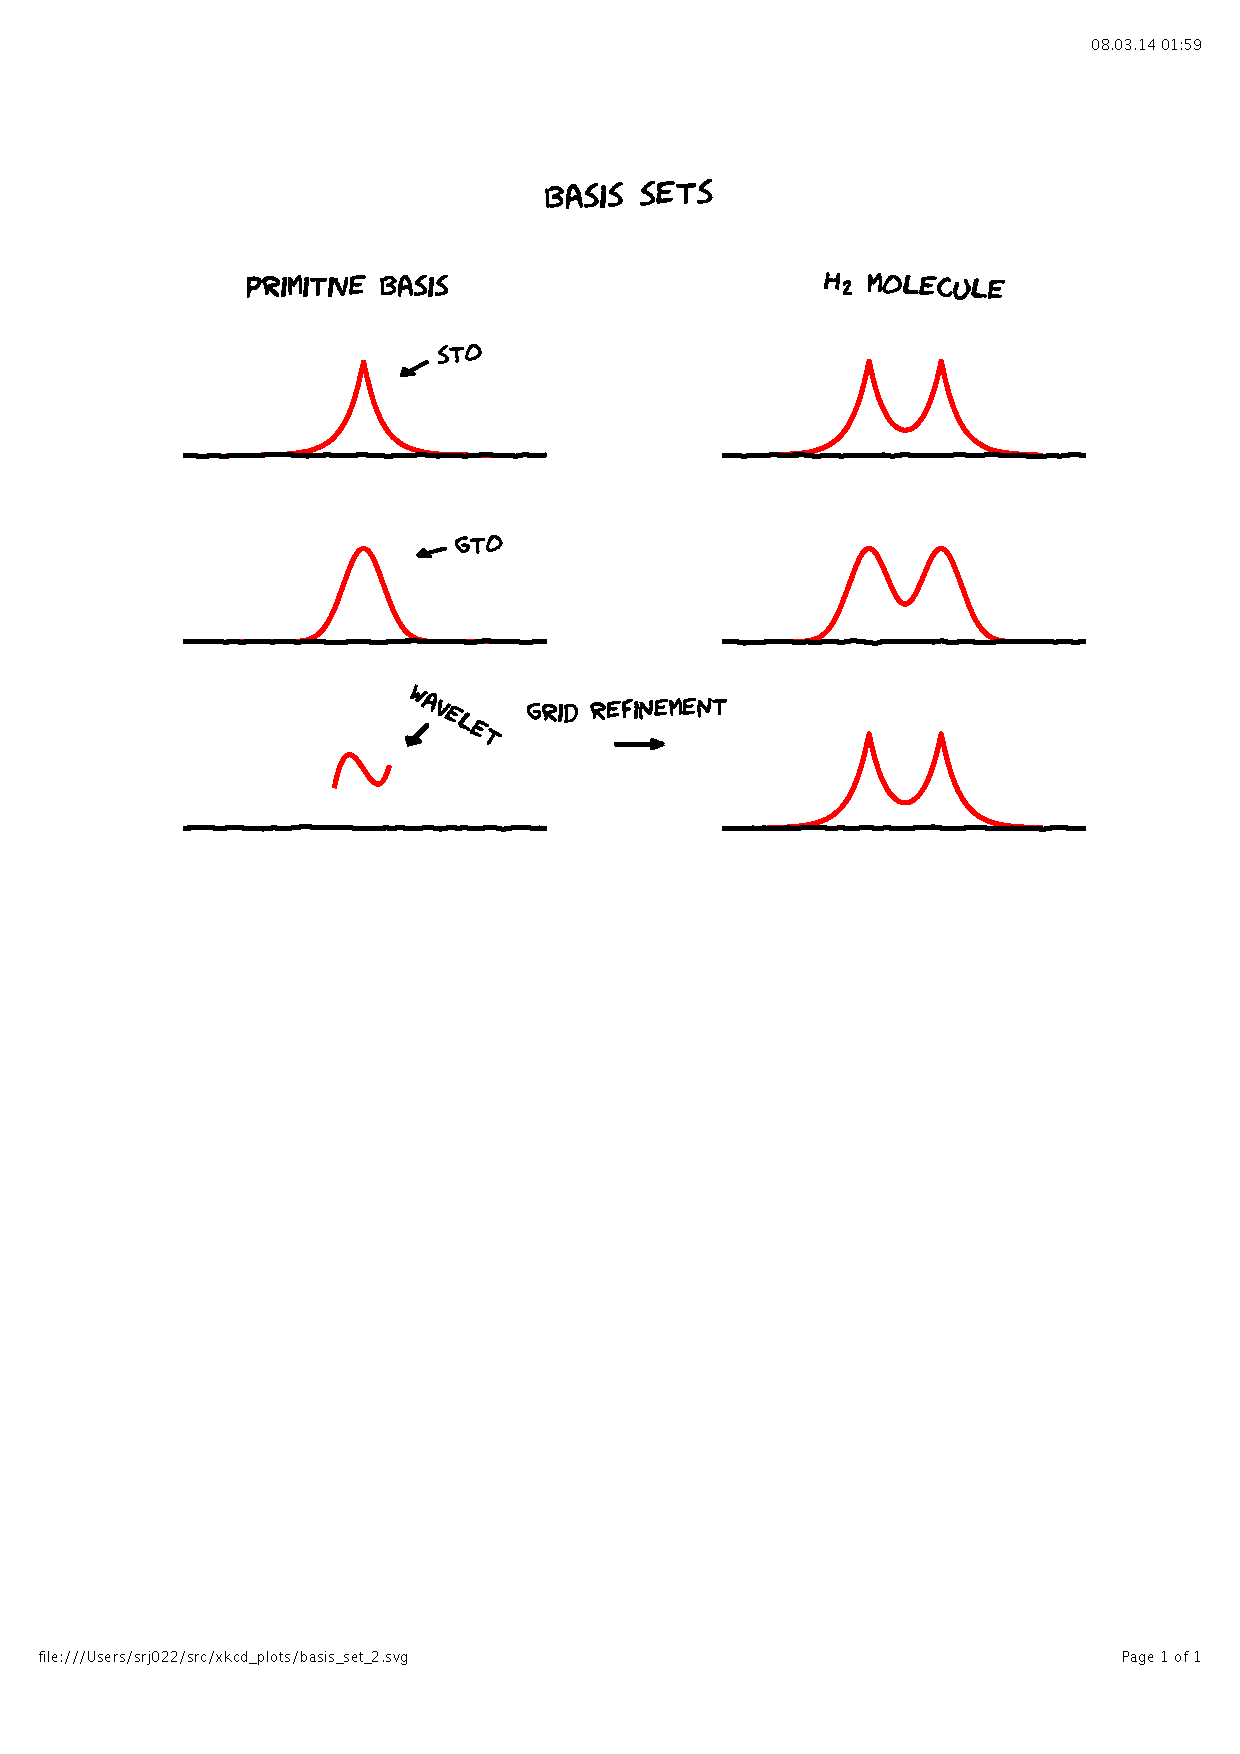
\includegraphics[scale=0.6, clip, viewport = 50 435 550 515]{figures/basis_set_2.pdf}}
    \end{center}
\end{frame}

\begin{frame}
    \frametitle{Integral formulation SCF}
    \centering
    \textbf{Kohn-Sham equations}
    \begin{equation}
	\nonumber
	\bigg[-\frac{1}{2}\nabla^2 + \hat{V}\bigg]\orbital_i(r) = \epsilon_i \orbital_i(r)
    \end{equation}

    \vspace{5mm}

    \textbf{Rewrite using} $\mu_i^2 = -2\epsilon_i$
    \begin{align}
	\nonumber
	\Big[-\nabla^2 + \mu_i^2\Big]\orbital_i(r) =&\ -2\hat{V}\orbital_i(r)\\
	\nonumber
	\orbital_i(r) =&-2\Big[-\nabla^2 + \mu_i^2\Big]^{-1}\hat{V}\orbital_i(r)\\
	\nonumber
	\orbital_i =&-2\hat{G}_i\Big[\hat{V}\orbital_i\Big]
    \end{align}

    \vspace{5mm}

    \textbf{Bound-State Helmholtz operator}
    \begin{equation}
	\nonumber
	\hat{G}_if(r) = \int \frac{e^{-\mu_i |r-r'|}}{4\pi|r-r'|}f(r')dr'
    \end{equation}

    \vspace{5mm}

    \centering
    \tiny
    MH Kalos,
    {\it Phys. Rev.}, 
    \textbf{128(4)},
    1791 (1962)\\
    RJ Harrison, GI Fann, T Yanai, Z Gan and G Beylkin,
    {\it J. Chem. Phys.}, 
    \textbf{121},
    11587 (2004)
\end{frame}

%\begin{frame}
%    \frametitle{Total energy calculation}
%    \centering
%    \textbf{Kohn-Sham energy expression}
%    \begin{equation}
%        \nonumber
%        E[\rho] = T_s[\rho] + V_{en}[\rho] + J[\rho] + E_{xc}[\rho]
%    \end{equation}
%
%    \vspace{3mm}
%
%    \textbf{Closed-shell system}
%    \begin{equation}
%        \nonumber
%        E = \sum_i^{N/2} 2\langle \orbital_i|\hat{T}|\orbital_i \rangle
%	    + \int \rho(r)v_{nuc}(r) \ud r
%	    + \frac{1}{2} \int \rho(r)v_{el}(r) \ud r
%	    + \int F_{xc} \ud r
%    \end{equation}
%
%    \vspace{3mm}
%
%    \textbf{Sum of orbital energies}
%    \begin{equation}
%        \nonumber
%        \sum_i^{N/2} 2\epsilon_i 
%	    = \sum_i^{N/2} 2\langle\orbital_i|\hat{T} + \hat{V}|\orbital_i\rangle
%	    = \sum_i^{N/2} 2\langle\orbital_i|\hat{T}|\orbital_i\rangle
%	        + \int \rho(r)\Big[v_{nuc}(r)+v_{el}(r)+v_{xc}(r)\Big] \ud r
%    \end{equation}
%
%    \vspace{3mm}
%
%    \textbf{Alternative expression}
%    \begin{equation}
%        \nonumber
%        E = 2 \sum_i^{N/2} \epsilon_i - \frac{1}{2} \int \rho(r)v_{el}(r) \ud r
%	    + \int F_{xc} \ud r - \int \rho(r)v_{xc}(r) \ud r
%    \end{equation}
%\end{frame}

